        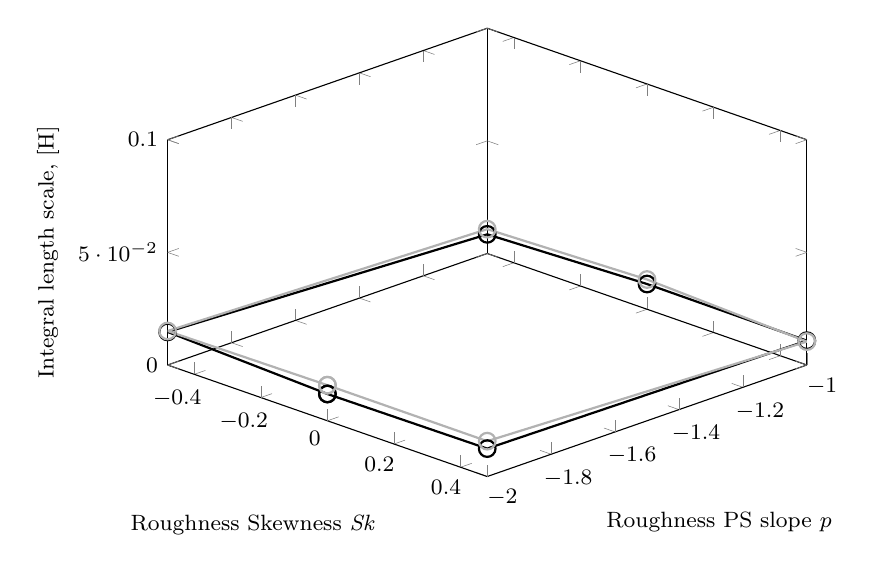
\begin{tikzpicture}[]
        \centering
        \begin{axis}[
        view={45}{35},
            ylabel={Roughness PS slope $p$},
            xlabel={Roughness Skewness \textit{Sk}},
			zlabel={Integral length scale, [H]},
			%ztick={0, 0.02,0.04,0.06,0.08},
			zmin=0,zmax=0.1,
            %ymin=0, ymax=0.16,
            width=.8\textwidth,
            height=.6\textwidth,
            label style={font=\footnotesize},
            tick label style={font=\footnotesize}
            ]
            
            
            
                                    \addplot3 [
            black,mark=o,thick, mark size=3pt
            ]
            coordinates{
            (0,-2,0.0119)			
			(0.48,-2,0.0124)
			(0.48,-1,0.0108)
			(0,-1,0.0112)
			(-0.48,-1,0.0085)
			(-0.48,-2,0.0147)
            (0,-2,0.0119)
			};
			\addplot3 [
            gray!60,mark=o,thick, mark size=3pt
            ]
            coordinates{
            (0,-2,0.0158)
			(0.48,-2,0.0157)
			(0.48,-1,0.0104)
			(0,-1,0.0132)
			(-0.48,-1,0.0108)
			(-0.48,-2,0.0151)
			(0,-2,0.0158)
            };
            
        \end{axis}
        \end{tikzpicture}